%!TEX root = ../notas_de_clase.tex

%%%%% NOMBRE ESCRIBAS Y FECHA
\newcommand{\sca}{Sebastian Bustos}
\newcommand{\scb}{Felipe Hernández}
\newcommand{\scc}{Nicolás Toro}
\newcommand{\catnum}{1} %numero de catedra
\newcommand{\fecha}{20 de marzo de 2020}

%%%%%%%%%%%%%%%%%%

%Macros para este documento
\newcommand{\cin}{\operatorname{cint}}


\begin{document}
%Encabezado

% notas al margen
% \ifnum \notasalmargen=1
% \newgeometry{left=1.5cm,top=1.5cm,right=1.5cm, bottom=1.5cm,letterpaper, includeheadfoot, outer=5cm, heightrounded, marginparwidth=4cm, marginparsep=-2.5cm}
% \fi
\NAM{
\newgeometry{left=1.5cm,top=1.5cm,right=1.5cm, bottom=1.5cm,letterpaper, includeheadfoot, outer=5cm, heightrounded, marginparwidth=4cm, marginparsep=-2.5cm}
\savegeometry{notas-al-margen}
}{}

%fin de notas al margen

\fancyhead[L]{Facultad de Ciencias Físicas y Matemáticas}
\fancyhead[R]{Universidad de Chile}
\vspace*{-1.2 cm}
\NAM{\begin{minipage}{0.7\textwidth}}{0.6\textwidth}
\begin{flushleft}
\hspace*{-0.5cm}\textbf{MA4702. Programación Lineal Mixta. 2020.}\\
\hspace*{-0.5cm}\textbf{Profesor:} José Soto\\
\hspace*{-0.5cm}\textbf{Escriba(s):} \sca, \scb ~y \scc.\\
\hspace*{-0.5cm}\textbf{Fecha:} \fecha.
\end{flushleft}
\end{minipage}
\NAM{\begin{minipage}{0.4\textwidth}}{\begin{minipage}{0.36\textwidth}}
\begin{flushright}
\NAM{\hspace*{4.3cm}
\includegraphics[scale=0.15]{fcfm}}{
\includegraphics[scale=0.15]{fcfm}}
\end{flushright}
\end{minipage}
\bigskip

\begin{center}
\LARGE\textbf{Cátedra \catnum}
\end{center}

%Fin encabezado

\section*{Introducción}

En esta sesión se estudiarán los conceptos formales de lo que es un problema de optimización en una forma general, se definirán conceptos claves para el trabajo de problemas de optimización con diferentes restricciones y se presentan ejemplos que ilustran lo presentado.


\section{Problemas y algoritmos (en optimización)}
Comencemos con las definiciones esenciales:

\begin{defi}[Problema de optimización e instancias]
Un \emph{problema de optimización} $\mathcal{P}$ es un conjunto de \emph{instancias}. Cada \emph{instancia} $\mathcal{I}$ esta definida por:
\begin{itemize}
    \item Un conjunto factible $S=\text{fact}(\mathcal{I})$.
    \item Una función a optimizar $f\colon S\to \RR$.
    \item Un objetivo, minimizar o maximizar   la función $f$ en dicho conjunto $S$.
\end{itemize}

\end{defi}
Usualmente las instancias se describen de manera implicita o compacta.

\begin{eje}[Árbol cubridor de peso mínimo -- minimum spanning tree, MST]
Cada instancia del problema (MST) se describe de manera compacta indicando un grafo $G=(V,E)$ con pesos en las aristas $w\colon E \to \RR_+$. De estos datos uno puede deducir el conjunto $S$ de todos los árboles cubridores de $G$, y para cada árbol $T\in \mathcal{S}$, el valor de la función es la suma de los pesos de las aristas $w(T)=\sum_{e\in E[T]}w(e)$. El objetivo es minimizar la función de peso $w$:
\[ \min\limits_{T\in S}~  w(T) \]
\end{eje}

\begin{defi}[Algoritmo] Un \emph{algoritmo} para un problema de optimización $\mathcal{P}$  es un método que recibe una instancia $(S,f,\max)$ y entrega, en un número finito de pasos:
\begin{enumerate}
    \item El óptimo en caso de existir. Es decir un elemento $\OPT \in S$ tal que $f\left(\OPT\right)= \displaystyle{\max_{x\in S}}~f(x)$.
    \item Ó bien certifica que no existe elemento óptimo. Esto puede pasar cuando:
        \begin{enumerate}
            \item El problema es infactible $\left(S=\emptyset\right)$.
            \item El problema no es acotado $\left(\displaystyle{\max_{x \in S}}~f(x)= \infty\right)$.
            \item El maximo no se alcanza $\left(\max \neq \sup\right)$.
        \end{enumerate}
\end{enumerate}
\end{defi}

Diremos que un algoritmo que siga la estructura anterior resuelve el problema de optimización.

\begin{eje}[Kruskal -- MST]
Un ejemplo de un algoritmo que resuelve el problema MST es Kruskal, modificándolo previamente  para que certifique que no hay solución al problema si es que el grafo es disconexo.
\end{eje}

Es importante notar que un algoritmo \textbf{tiene} que terminar en un tiempo finito (en la practica, el tiempo de ejecución puede ser tan grande, que no hay diferencia entre esto e ``infinito'').

\newpage

\section{Programas Lineales Mixtos}

\begin{defi}[Conjunto lineal mixto] Se dice que $S \subseteq \ZZ^{E} \times \RR^{C} \subseteq \RR^{n}$ es un conjunto lineal mixto si $S$ pude ser descrito como intersección de un conjunto finito de desigualdades lineales. Es decir $S$ es:
\[
S:=\{x \in \ZZ^{E} \times \RR^{C} : Ax \leq b\} \subseteq \RR^{n}.
\]

Con $n,m \in \NN$, $E,C \subseteq [n]$ tales que $E \cup C = [n]$, $A \in \mathcal{M}_{m \times n}(\RR)$ y $b \in \RR^{m}$.

La interpretación y nombres en la definición de un conjunto lineal mixto viene dado por:

\begin{enumerate}
    \item Las coordenadas en $E$ se llaman \emph{variables enteras}.
    \item Las coordenadas en $C$ se llaman \emph{variables continuas}.
    \item Las $m$ desigualdades de la forma $a_{j}^{T}x \leq b_{j}$ se llaman \emph{restricciones}.
    \item Si $E=[n]$ a $S$ se le llama \emph{conjunto lineal entero}.
    \item Si $C=[n]$ a $S$ se le llama \emph{conjunto lineal puro o poliedro}.
    \item Si $x \in \{0,1\}^{n}$ a $S$ se le llama \emph{conjunto lineal binario}.
\end{enumerate}
\end{defi}


\begin{eje}

En la Figura 1 podemos ver un conjunto lineal puro en $\RR^2$, el cual esta determinado por las inecuaciones:
$$\begin{pmatrix}    
0\\ 
0\\
y\\ 
\end{pmatrix}\leq\begin{pmatrix}    
y\\ 
x\\
c-x\\ 
\end{pmatrix},
$$
donde $c>0$. Mientras que en la Figura 2 observamos el conjunto lineal mixto obtenido añadiendo la restricción adicional $x\in \ZZ$.

Es importante recordar que sin perder generalidad se puede suponer que $Ax \leq b$ incluye todas las restricciones lineales de un problema de optimización (tanto las inecuaciones como las igualdades).

En la Figura 3 podemos observar un conjunto lineal binario, que cumple la restricción $x \in \{0,1\}^3$
\begin{figure}[h!]
    \centering
    \begin{minipage}{0.45\textwidth}
        \centering
        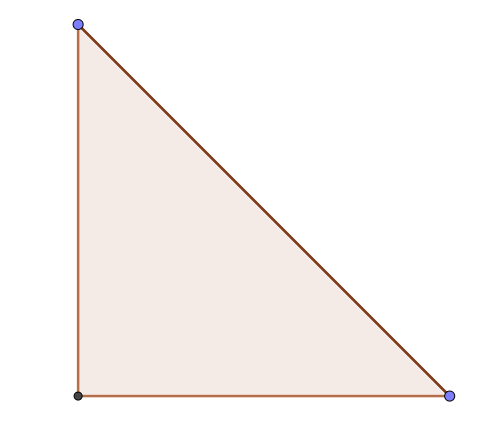
\includegraphics[width=0.7\textwidth]{Img1.PNG} % first figure itself
        \caption{Conjunto lineal puro}
    \end{minipage}\hfill
    \begin{minipage}{0.45\textwidth}
        \centering
        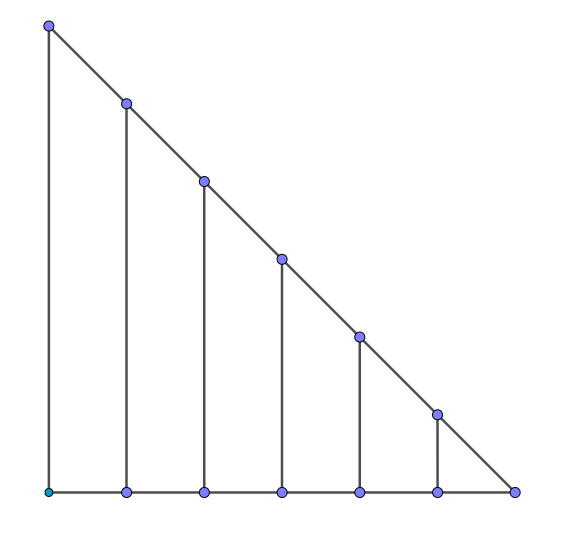
\includegraphics[width=0.65\textwidth]{Img2.PNG} % second figure itself
        \caption{Conjunto lineal mixto \newline \hspace*{1.5cm} Eje x variable entera \newline \hspace*{1.5cm} Eje y variable continua}
    \end{minipage}
    %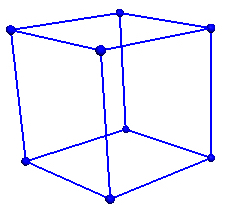
\includegraphics[width=0.3\textwidth]{cube3.jpg}
    %\caption{Conjunto lineal binario}
\end{figure}

\end{eje}
\newpage
\begin{figure}
    \centering
    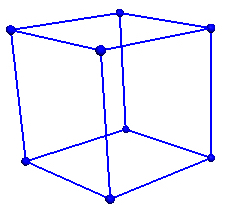
\includegraphics[width=0.3\textwidth]{cube3.jpg}
    \caption{Conjunto lineal binario}
\end{figure}
\begin{defi}[Programas lineales puros / mixtos / enteros / binarios] Diremos que un problema de la forma:
$$
\max\{c^{t}\colon x \in S\}
$$
es un \emph{programa lineal puro / mixto / entero / binario} si $S$ es un conjunto lineal puro / mixto / entero / binario. 
\end{defi}

Se abreviaran como \emph{PL / PLM / PLE / PLB} respectivamente.

\textbf{Observación:} A $S$ se le conoce como dominio o conjunto factible del programa.
\section{Modelos}

En general los problemas de optimización que aparecen en la vida real no están escritos como un PLM. Por ende es necesario reescribir un problema para poder trabajarlo como tal.

\begin{defi}[Modelo] Diremos que un PLM es modelo de un problema si

\begin{itemize}
    \item Cada solución óptima del PLM es solución óptima del problema original.
    \item Al menos una solución óptima del problema original es factible en el PLM
\end{itemize}
\end{defi}

Es importante notar que a veces se relaja la primera condición y se pide que sea algún tipo de solución óptima en particular. La definición anterior da la oportunidad de que existan soluciones óptimas del problema original que no sean factibles en el PLM, en caso contrario nos encontramos frente a un modelo particular:

\begin{defi}[Modelo exacto] Diremos que un PLM es un modelo exacto si las soluciones factibles del problema original están en correspondencia uno a uno, de manera explicita con las soluciones factibles del PLM
\end{defi}

\begin{eje}[Knapsack/ Problema de la mochila] Dado $n \in \NN$ objetos, valores $v_{i} \geq 0$ y tamaños $s_{i} \geq 0$. Dada una mochila de capacidad $B \geq 0$. Seleccionar un subconjunto a poner en la mochila maximizando el valor total.

\begin{equation*}
\begin{aligned}
\textrm{(Knapsack)}~ & \max
& & \displaystyle{\sum_{i \in [n]}}~v_{i}x_{i}\\
& \text{s.a.}
& & \displaystyle{\sum_{i \in [n]}}~s_{i}x_{i} \leq B\\
&&& x_{i} \in\{0,1\} ~ \forall i \in [n],
\end{aligned}
\end{equation*}
\newpage
donde
\begin{enumerate}
    \item $x_{i}=1 \iff i \text{  se encuentra en la mochila}$
    \item $\displaystyle{\sum_{i \in [n]}}~s_{i}x_{i}$ es la capacidad ocupada de la mochila.
    \item $\displaystyle{\sum_{i \in [n]}}~v_{i}x_{i}$ es el valor de la mochila.
\end{enumerate}

\end{eje}

\textbf{Observación 1:} Este modelo es exacto.

\textbf{Observación 2:} Es importante notar que a veces, por mucho que se conozcan técnicas para resolver un problema, es conveniente escribir el problema como un PLM, lo anterior permite la libertad de agregar restricciones fácilmente a los problemas de optimización.

\begin{eje}[s-t Camino de largo mínimo] Dado el digrafo $G=(V,\Vec{E})$, nodo de origen $s \in V$, nodo destino $t \in V$. Dada además una función de largos no negativos $\ell: \Vec{E} \to \RR_{+}$. Determinar un camino de largo mínimo de $s$ a $t$. Para resolver este problema, necesitamos caracterizar de alguna manera los $s$-$t$ caminos.  Veremos dos maneras de realizar esto:
\begin{enumerate}[\bf I.-]
    \item \textbf{(Mediante cortes)} Sea $x\in \{0,1\}^E$ en donde $\forall e\in E, ~x(e)=1 \iff$ el arco $e$ esta siendo ocupado.\\
    Recordemos la definición de corte:
    \begin{defi}[s-t corte] Un subconjunto $U \subseteq V$ es un $s$-$t$ corte si $s \in U, t \not \in U$. 
    \end{defi}
    Tambien recordemos las siguientes definiciones:
    \begin{defi}
    \hphantom{0.5 cm}
    \begin{itemize}
        \item $\delta^{+}(U)$ son los arcos que salen del conjunto $U$.
        \item $\delta^{-}(U)$ son los arcos que entran del conjunto $U$. 
    \end{itemize} 
    \end{defi}
    Para caracterizar que se sale de cada $U$ $s$-$t$ corte utilizaremos la siguiente ecuación:
    $$x(\delta^+(U)):= \sum\limits_{e\in \delta^+(U)} x(e) \geq 1 $$
    Así el problema lo podemos plantear como sigue:

\begin{equation*}
\begin{aligned}
\textrm{(SP-Conector)}~ & \min
& & \displaystyle{\sum_{e \in E}}~\ell_{e}x_{e}\\
& \text{s.a.}
& & x\left(\delta^{+}(U)\right) \geq 1 \text{ para todo }s\text{-}t \text{ corte } U \\
&&& x \in\{0,1\}^{E}
\end{aligned}
\end{equation*}


\begin{enumerate}
    \item Se puede probar que si el conjunto de arcos cruza todos los cortes entonces tiene que haber un $s$-$t$ camino.
    \item Hay $|\mathcal{P}(V\setminus\{s,t\})|=2^{n-2}$ cortes, y por ende $2^{n-2}$ restricciones.
\end{enumerate}
Se dejan los siguientes ejercicios propuestos:

\begin{ejer}
Probar que para el problema $s$-$t$ camino de coste mínimo y $\ell_e{} >0 ~ \forall e$ entonces SP-Conector es un modelo. Y probar que (en general) no es un modelo exacto.
\end{ejer}
\begin{ejer}
Modificar SP-Conector para que incluso cuando $\ell$ pueda tomar valores nulos sea un modelo.
\end{ejer}
\vspace{0.1 mm}
Es importante notar que la cantidad de restricciones crece de manera exponencial con el tamaño, luego, si bien el modelo soluciona el problema, en la practica el tiempo en que se ejecute el programa va a ser grande.

Por lo anterior es conveniente plantear el problema de otra manera. 

\newpage
    \item \textbf{(Mediante flujos)} Recordemos la definición de flujo: 
    
    
\begin{defi}[s-t flujo] Una función $f:E \to \RR_{+}$ es un $s$-$t$ flujo si:

$$
f\left(\delta^{+}(u)\right)=f\left(\delta^{-}(u)\right) ~ \forall u \in V \backslash\{t,s\}
$$
\end{defi}
Luego el problema es posible plantearlo como:

\begin{equation*}
\begin{aligned}
\textrm{(SP-Flujo)}~ & \min
& & \displaystyle{\sum_{e \in E}}~\ell_{e}x_{e}\\
& \text{s.a.}
& & x(\delta^{+}(u))=x(\delta^{-}(u))~ \forall u \in V \backslash\{t,s\} \\
&&& x(\delta^{+}(s))=x(\delta^{-}(t))=1\\
&&& x(\delta^{-}(s))=x(\delta^{+}(t))=0\\
&&& x \in\{0,1\}^{E}
\end{aligned}
\end{equation*}


De esta manera existen $n+2$ restricciones lo cual es una cantidad lineal de restricciones.

\begin{ejer}
Verifique que SP-Flujo es un modelo del problema cuando $\ell_{e} >0 ~\forall e$ y muestre que, en general, no es un modelo exacto.
\end{ejer}
\begin{ejer}
Modifique SP-Flujo para que sea un modelo incluso cuando $\ell$ pueda tomar valores nulos.
\end{ejer}

\begin{ejer}Pruebe que SP-Flujo es equivalente a

\begin{equation*}
\begin{aligned}
& \min
& & \displaystyle{\sum_{e \in E}}~\ell_{e}x_{e}\\
& \text{s.a.}
& & x(\delta^{+}(u))=x(\delta^{-}(u))~ \forall u \in V \backslash\{t,s\} \\
&&& x(\delta^{+}(s))-x(\delta^{-}(s))=1\\
&&& x \in\{0,1\}^{E}
\end{aligned}
\end{equation*}


\end{ejer}
    
\end{enumerate}

Mostraremos en el curso que el problema es posible relajarse y en vez de considerar $x\in \{0,1\}^{E}$ se puede transformar al problema lineal puro con la restricción  $0 \leq x \leq 1$.




\end{eje}


\end{document}

%%%%%%%%%%%%%%%%%%%%%%%%%%%%%%%%%%%%%%%%%%%%%%%%%%%%%%%%%%%%%%%%%%%%%%%%%%%%%%%%%%%%%%%%%%%%
%%%%%%%%%%%%%%%%%%%%%%%%%%%%%%%%%%%%%%%%%%%%%%%%%%%%%%%%%%%%%%%%%%%%%%%%%%%%%%%%%%%%%%%%%%%%